\documentclass[../../main.tex]{subfiles}
\begin{document}

% Results
    % Tables
    % Comparable images
% Analysis
    % What does out data mean
    % Why do we get the results we do?


%%%%%%%%
\section{Implementation}
%%%%%%%%

During our implementation we used the visual C++ 12.0 compiler on Windows 8.1 OS and compiled towards 64-bit. Our tests consisted of running simulations until 10 seconds of real time had been simulated. Throughout the tests we varied the scene complexity and particle count. The tests were performed on computers with 16 gigabyte of memory, Intel Core i7-2700K processors (3.5 GHz, 8 cores) and were multithreaded using OpenMP. 

In all tests we used static boundary particles for walls and collision objects for the simplicity when it comes to implementation. 

\begin{figure}[h!]
    \centering
    \includegraphics[width=\textwidth]{Comparison.png}
    \caption[Visual comparison of the algorithms]{A visual comparison of the four algorithms (from the top: PCISPH, two-scale, RTS, and finally our combined). The scene is \textit{double dam break with pillars} and the screen shots are taken at the times 0.3s, 1.6s, 3.3s, and 5.0s. }
    \label{fig:comparison}
\end{figure}

%%%%%%%%
\section{Results}
%%%%%%%%

As can be seen in tables \ref{table:gallery} through \ref{table:pillars}, our combined method is not as fast as one might have expected. However, our two-scale implementation has not given the speedup over PCISPH as shown in Solenthaler's paper. We believe this could be caused by a couple of discrepancies. Firstly, the resolution factor in our implementation is only 2, whereas in the two-scale paper it is in some tests set to 4. A resolution factor of 4 gives L-particles which are 64 times larger than the H-particles, reducing the total number of particles significantly. Secondly, our scenes and specifically the determination of the H-regions differs a bit. Our regions are up to 50\% of the whole simulation domain, and Solenthaler's seem to be around 25\% in most of the scenes. Because of the amount of active particles, the overhead from certain calculations (create/delete H-particles, boundary handling, parent update) might outweigh the benefits of the two-scale method. 


The RTS algorithm is not as sensitive to scene configuration as the two-scale algorithm. 
%Therefore, we can assume that the speed up we see in our combined algorithm comes from RTS. 
Therefore, we see the same speed up in the results from our combined algorithm as the RTS has over PCISPH. 

Visually, we see few discrepancies between the algorithms, as is made clear in figure \ref{fig:comparison}. There is, of course, some difference between the L-area in two-scale and the combined algorithm, and the corresponding area in PCISPH and RTS, but that is to be expected from the two-scale base algorithm. 

\begin{table}[]
\centering
\caption{Simulation results from the Gallery scene}
\label{table:gallery}
\begin{tabular}{llll}
\hline
Technique & Particle count      & Time (s) & Speedup \\ \hline
PCISPH    & 1.1M                & 54343.5  & -       \\
Two-scale & L: 140k H: 400-600k & 54923.5  & 0.989   \\
RTS       & 1.1M                & 47750.7  & 1.138   \\
Combined  & L: 144k H: 400-600k & 45385.8  & 1.197   \\ \hline
\end{tabular}
\end{table}


\begin{table}[]
\centering
\caption{Simulation results from the Double dam break scene}
\label{table:doubledam}
\begin{tabular}{llll}
\hline
Technique & Particle count      & Time (s) & Speedup \\ \hline
PCISPH    & 950k                & 45486.4  & -       \\
Two-scale & L: 120k H: 300-500k & 105931   & 0.429   \\
RTS       & 950k                & 40519    & 1.123   \\
Combined  & L: 120k H: 300-500k & 42342.4  & 1.197   \\ \hline
\end{tabular}
\end{table}

\begin{table}[]
\centering
\caption{Simulation results from the Double dam break with pillars scene}
\label{table:pillars}
\begin{tabular}{llll}
\hline
Technique & Particle count      & Time (s) & Speedup \\ \hline
PCISPH    & 950k                & 47172    & -       \\
Two-scale & L: 120k H: 300-570k & 117816   & 0.400   \\
RTS       & 950k                & 41841    & 1.127   \\
Combined  & L: 120k H: 300-570k & 40642.8  & 1.074   \\ \hline
\end{tabular}
\end{table}


\begin{table}[]
\centering
\caption{Time distribution over all parts in the combined algorithm}
\label{table:timedistribution}
\begin{tabular}{cccll}
\hline
\begin{tabular}[c]{@{}c@{}}Pre-Minor \\ L\end{tabular} & Determine Region & \begin{tabular}[c]{@{}c@{}}Pre-Minor\\ H\end{tabular} & \textbf{Minor steps}                 & Update Parent              \\ \hline
1.30\%                                                 & 17.70\%          & 7.40\%                                                & \multicolumn{1}{c}{70.50\%} & \multicolumn{1}{c}{3.00\%} \\ \hline
\end{tabular}
\end{table}


\begin{table}[]
\centering
\caption{Minor step time details}
\label{table:minordetails}
\begin{tabular}{ccccccc}
\hline
L                           & \multicolumn{5}{c}{H}                                                                                                                                                                                                                                                                      & Feedback             \\ \hline
\multicolumn{1}{c|}{}       & \multicolumn{5}{c|}{91.00\%}                                                                                                                                                                                                                                                                &                      \\ \cline{2-6}
\multicolumn{1}{c|}{7.90\%} & \begin{tabular}[c]{@{}c@{}}Update \\ neighborhood\end{tabular} & \begin{tabular}[c]{@{}c@{}}Update\\ density\end{tabular} & \begin{tabular}[c]{@{}c@{}}Prediction \\ correction\end{tabular} & \begin{tabular}[c]{@{}c@{}}Update vel \\ and pos\end{tabular} & \multicolumn{1}{c|}{Other}  & 1.10\%               \\ \cline{2-6}
\multicolumn{1}{l|}{}       & 36.60\%                                                        & 7.20\%                                                   & 46.00\%                                                          & 4.70\%                                                        & \multicolumn{1}{c|}{5.50\%} & \multicolumn{1}{l}{} \\ \hline
\end{tabular}
\end{table}



%%%%%%%%
\section{Discussion}
%%%%%%%%

During our implementation we had some difficulties with the boundary and relaxed H-particles for the two-scale algorithm and therefore our combined algorithm. It is possible that there still exists some problems which causes the particles to get incorrect densities which in turn requires more iterations in the prediction-correction loop. The fact that most of the $\Re_1$ regions exist near the border (as can be seen in figure \ref{fig:redarea}) further supports this theory. 

In some tests, however, we see that our combined algorithm is faster than RTS and PCISPH, despite that the two-scale results shows much longer simulation time than PCISPH. This indicates that if our scenes were correctly set up and our two-scale implementation gave the same speed up as in the original paper, we would see a large speed up in our combined algorithm as well. 


\begin{figure}[h]
    \centering
    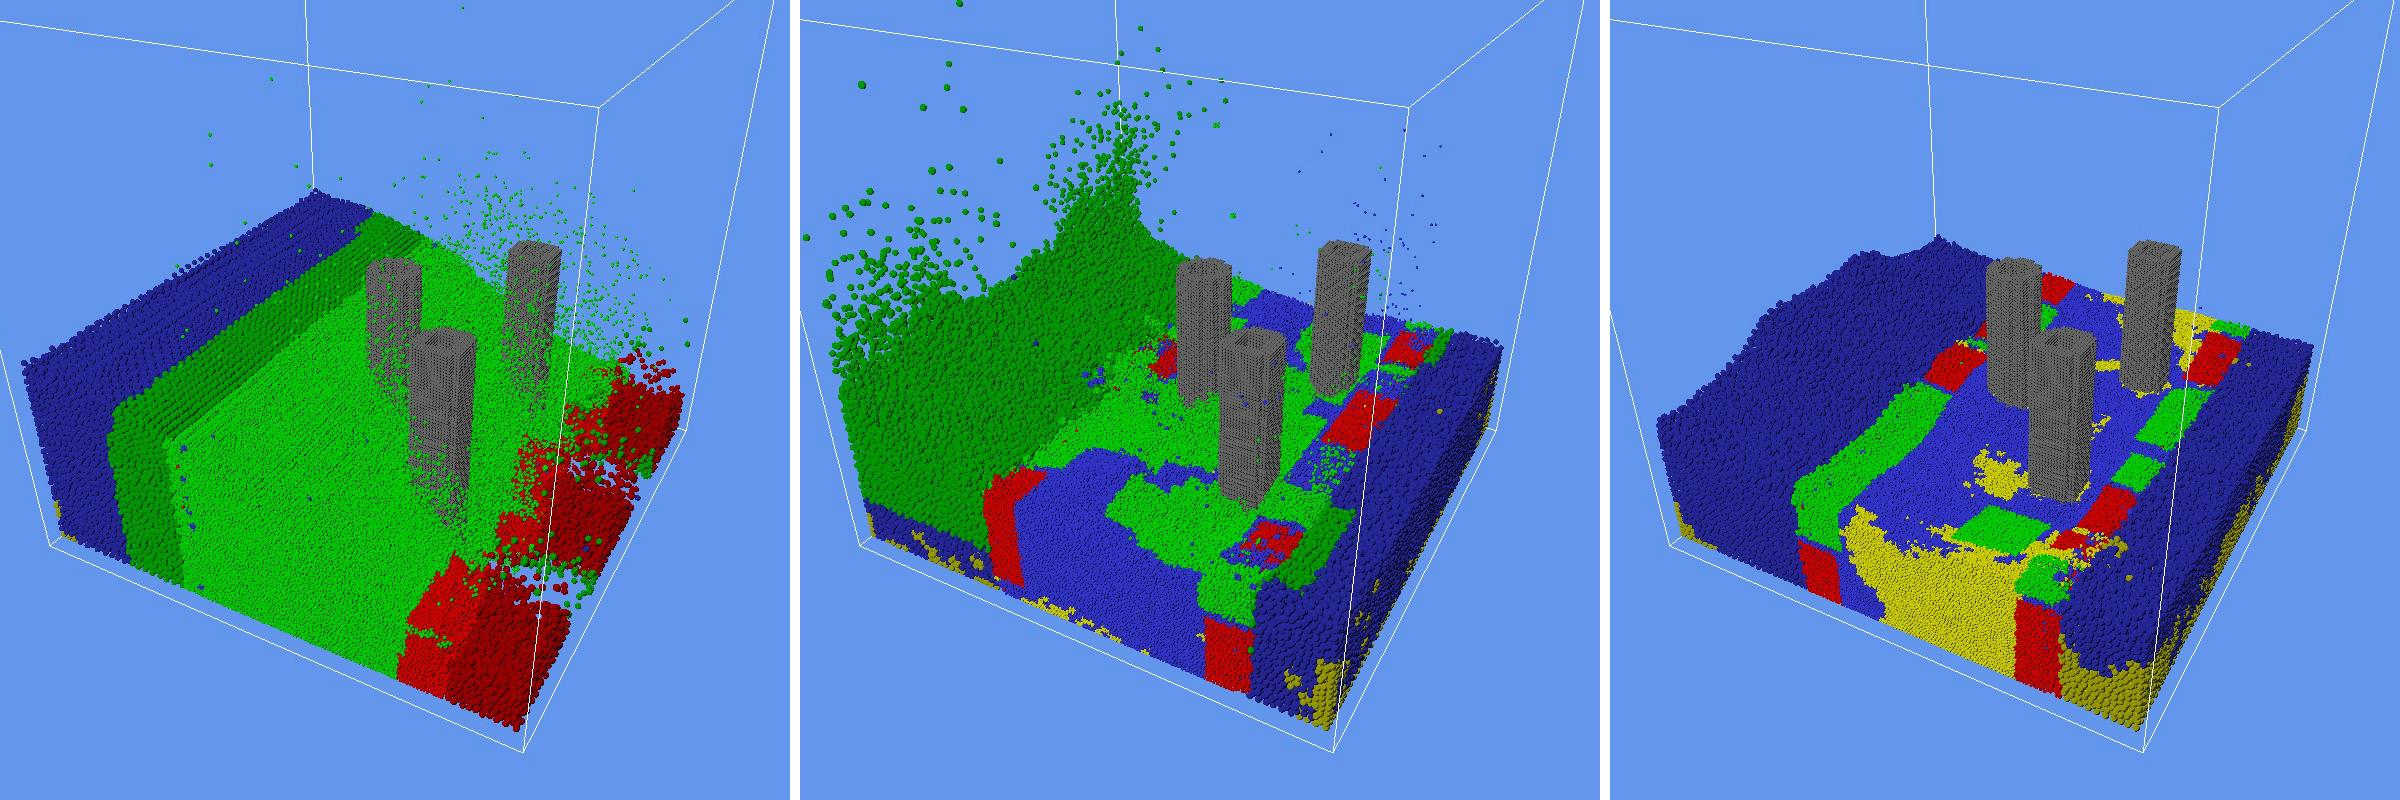
\includegraphics[width=\textwidth]{RedArea.png}
    \caption[Lower time step along the border]{The $\Re_1$ area (colored red) is prominent along the border between H and L. }
    \label{fig:redarea}
\end{figure}



\end{document}